% mainfile: ../../../../master.tex
\subsection{Checking integrity of nucleic acids on agarose gel}
% The part of the label after the colon must match the file name. Otherwise,
% conditional compilation based on task labels does NOT work.
\label{task:20180315_cj2}
\tags{lab,dna,rna}
\authors{cj}
%\files{}
%\persons{}

\subsubsection{Introduction}

The first DNA and RNA quality parameters assessed earlier were based on DNA 260/280 and 260/230 spectrophotometric ratios measured by NanoDrop\cR ND-1000 and detectability by PCR. Another important quality parameters is the size range and integrity. Integrity does not mean purity. It means intactness or state of degradation of nucleic acids. DNA and RNA integrity and size range can be assessed by agarose gel electrophoresis.\sidenote{The size of my expected DNA would determine what percentage agarose gel should be used. Usually 0.8\% to 1\% will be good enough to see how degraded is the DNA or RNA.}

I have previously tried to test the integrity of nucleic acid with SYBR\cR Safe stain, but unfortunately SYBR\cR Safe did not stain my RNA samples. Therefore, I want to repeat this experiment with SYBR\cR Gold. SYBR\cR Gold is a very sensitive stain for detecting double- and single-stranded DNA or RNA in electrophoretic gels. 

\subsubsection{1\% Agarose gel preparation}

\begin{enumerate}
\item Measure with erlenmeyer 50~mL of 1\% agarose gel.\sidenote{The 1\% agarose gel is kept at 60\degree C in the gel room.}
\item Warm up the erlenmeyer for 15s in microwave: agarose will be more fluid and it will avoid bubbles when casting the gel
\item Cast the gel with the comb (for 15 wells)
\item Let the gel set for 20 min
\end{enumerate}

\subsubsection{Nucleic acid samples preparation}

\begin{itemize}
\item 5~\textmu L of each sample of nucleic acid sample
\item 5~\textmu L of blue dye (bromothymol blue)
\item Tap gently tubes to mix up everything
\item Centrifuge briefly to bring all the liquid to the bottom
\end{itemize}

\subsubsection{Electrophoresis}

For this electrophoresis migration, we run:
\begin{itemize}
\item 9~\textmu L of each sample 
\item 5~\textmu L of the 1~kb ladder
\item 5~\textmu L of the 2-log ladder
\end{itemize}
\comment{I leave empty lanes between ladders and samples.}

\begin{enumerate}
\item Place the agarose gel into the gel box (electrophoresis unit) containing TAE buffer
\item Load 5~\textmu L of molecular weight ladder into the first and last lane of the gel
\item Load 9~\textmu L of each sample into the additional wells of the gel
\item Run for 65 min with the \gls{eps} 301 at 80~V, 400~mA
\comment{I change the usual settings for a slightly longer run at a lowest voltage (the usual settings I use for electrophoresis are 50 min at 100~V), so that the separation of nucleic acid fragments will be slowlier but clearer.}
\item Remove gel from the migration tank and place in the staining container (a recycled tip box).
\end{enumerate}

\subsubsection{SYBR\cR Gold Staining}

\begin{enumerate}
\item Ensure SYBR\cR gold is properly thawed.
\item Ensure the pH of TAE buffer is between 7.5 and 8 (cf. figure \ref{sfig:20180315_TAE_pH_check})
\comment{I made a new batch of 10L of TAE buffer in the gel room thanks to Águsta.}
\item Prepare the staining solution at 1X SYBR\cR Gold in TAE buffer.
\comment{For 100 mL of staining solution, I mixed 10~\uL of SYBR\cR stain with 100 mL of TAE buffer.}
\item Transfer 100 mL of staining solution in the staining container.
\comment{I recycle a broken box of tips.}
\item Incubate under agitation for 10 to 40 min.
\comment{I incubated 20 min under 150 rpm at room temperature on the TITRAMAX 1000 by Heidolph (cf. figure \ref{sfig:20180315_sybr_gold_incubation})}
\item Visualize your nucleic acid fragments with \gls{uv} lights.
\end{enumerate}
\comment{Our usual CCD camera by BioRad does not work anymore. In the meanwhile, we use transilluminator and take the picture with my cell phone.}

\begin{figure}[H] % position of the figure 
    \centering
    \caption{SYBR\cR Gold Staining considerations and results}
    \label{fig:20180315_sybr_gold_staining}
    \begin{subfigure}[b]{0.37\textwidth}
        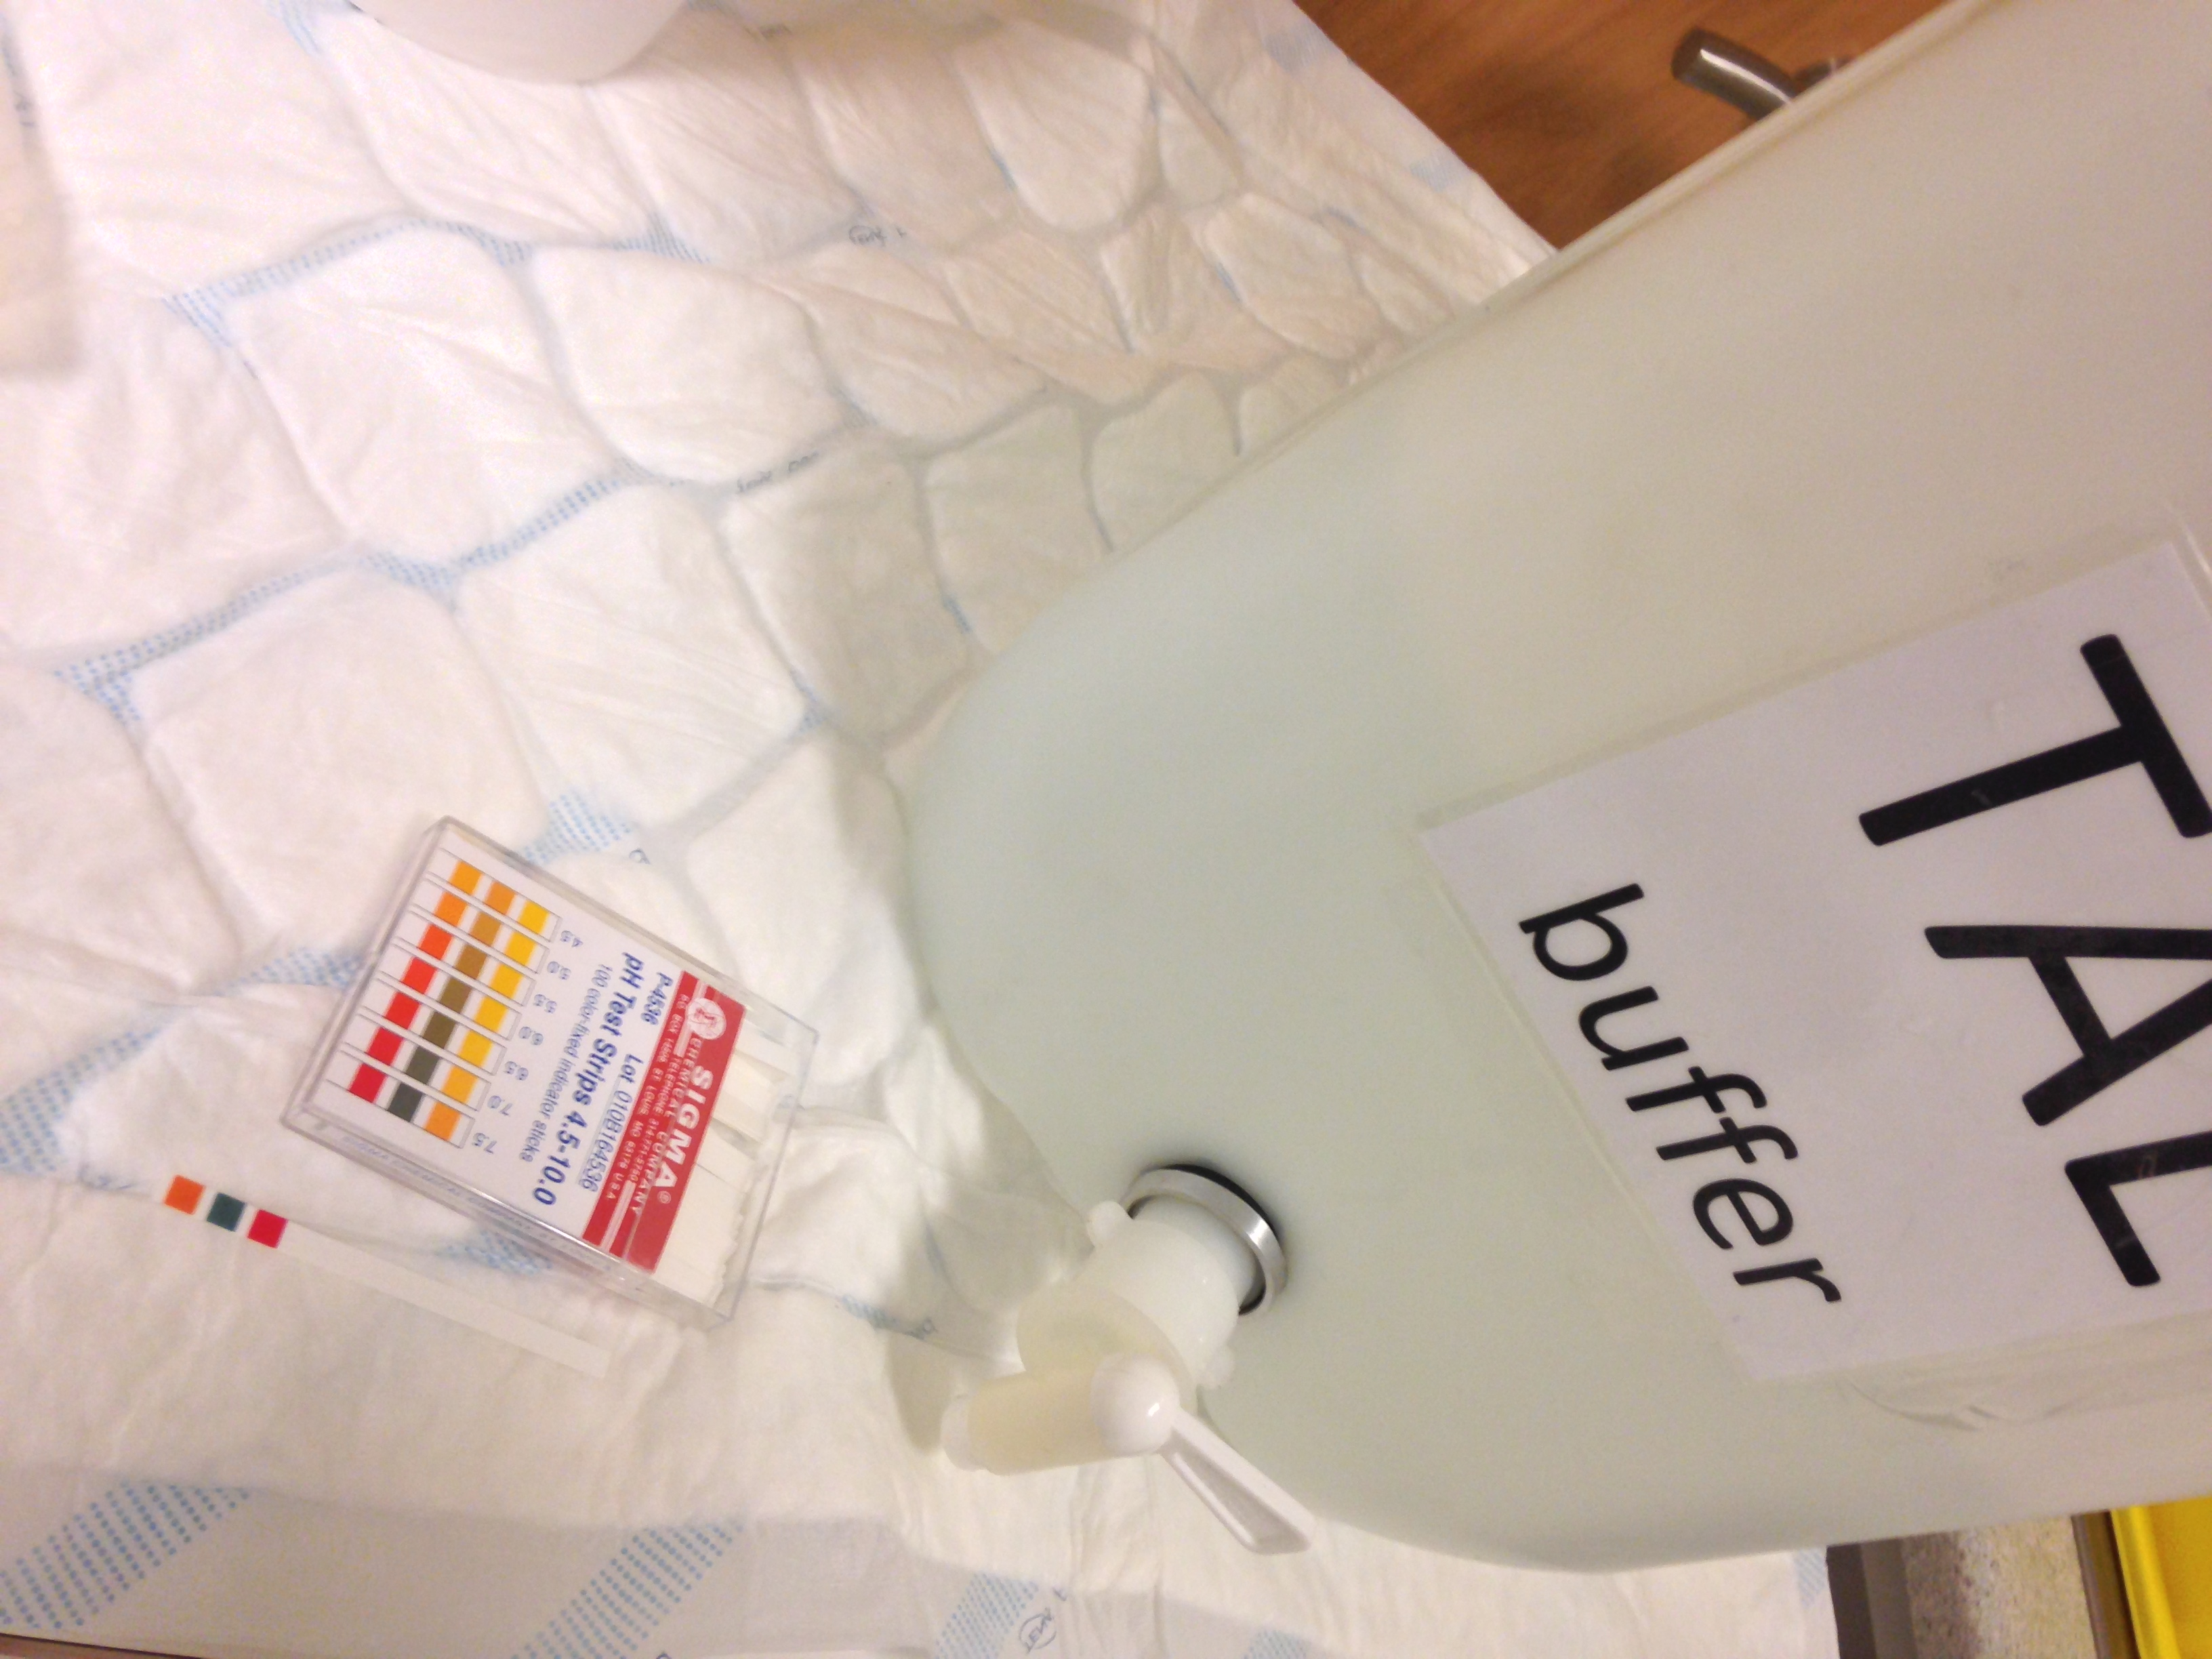
\includegraphics[width=\textwidth]{graphics/pic/20180315_TAE_pH_check.JPG}
        \caption{Ensure TAE buffer pH is between 7.5 and 8 because SYBR\cR Gold is pH sensitive}
        \label{sfig:20180315_TAE_pH_check}
    \end{subfigure}
    ~ 
    \begin{subfigure}[b]{0.37\textwidth}
        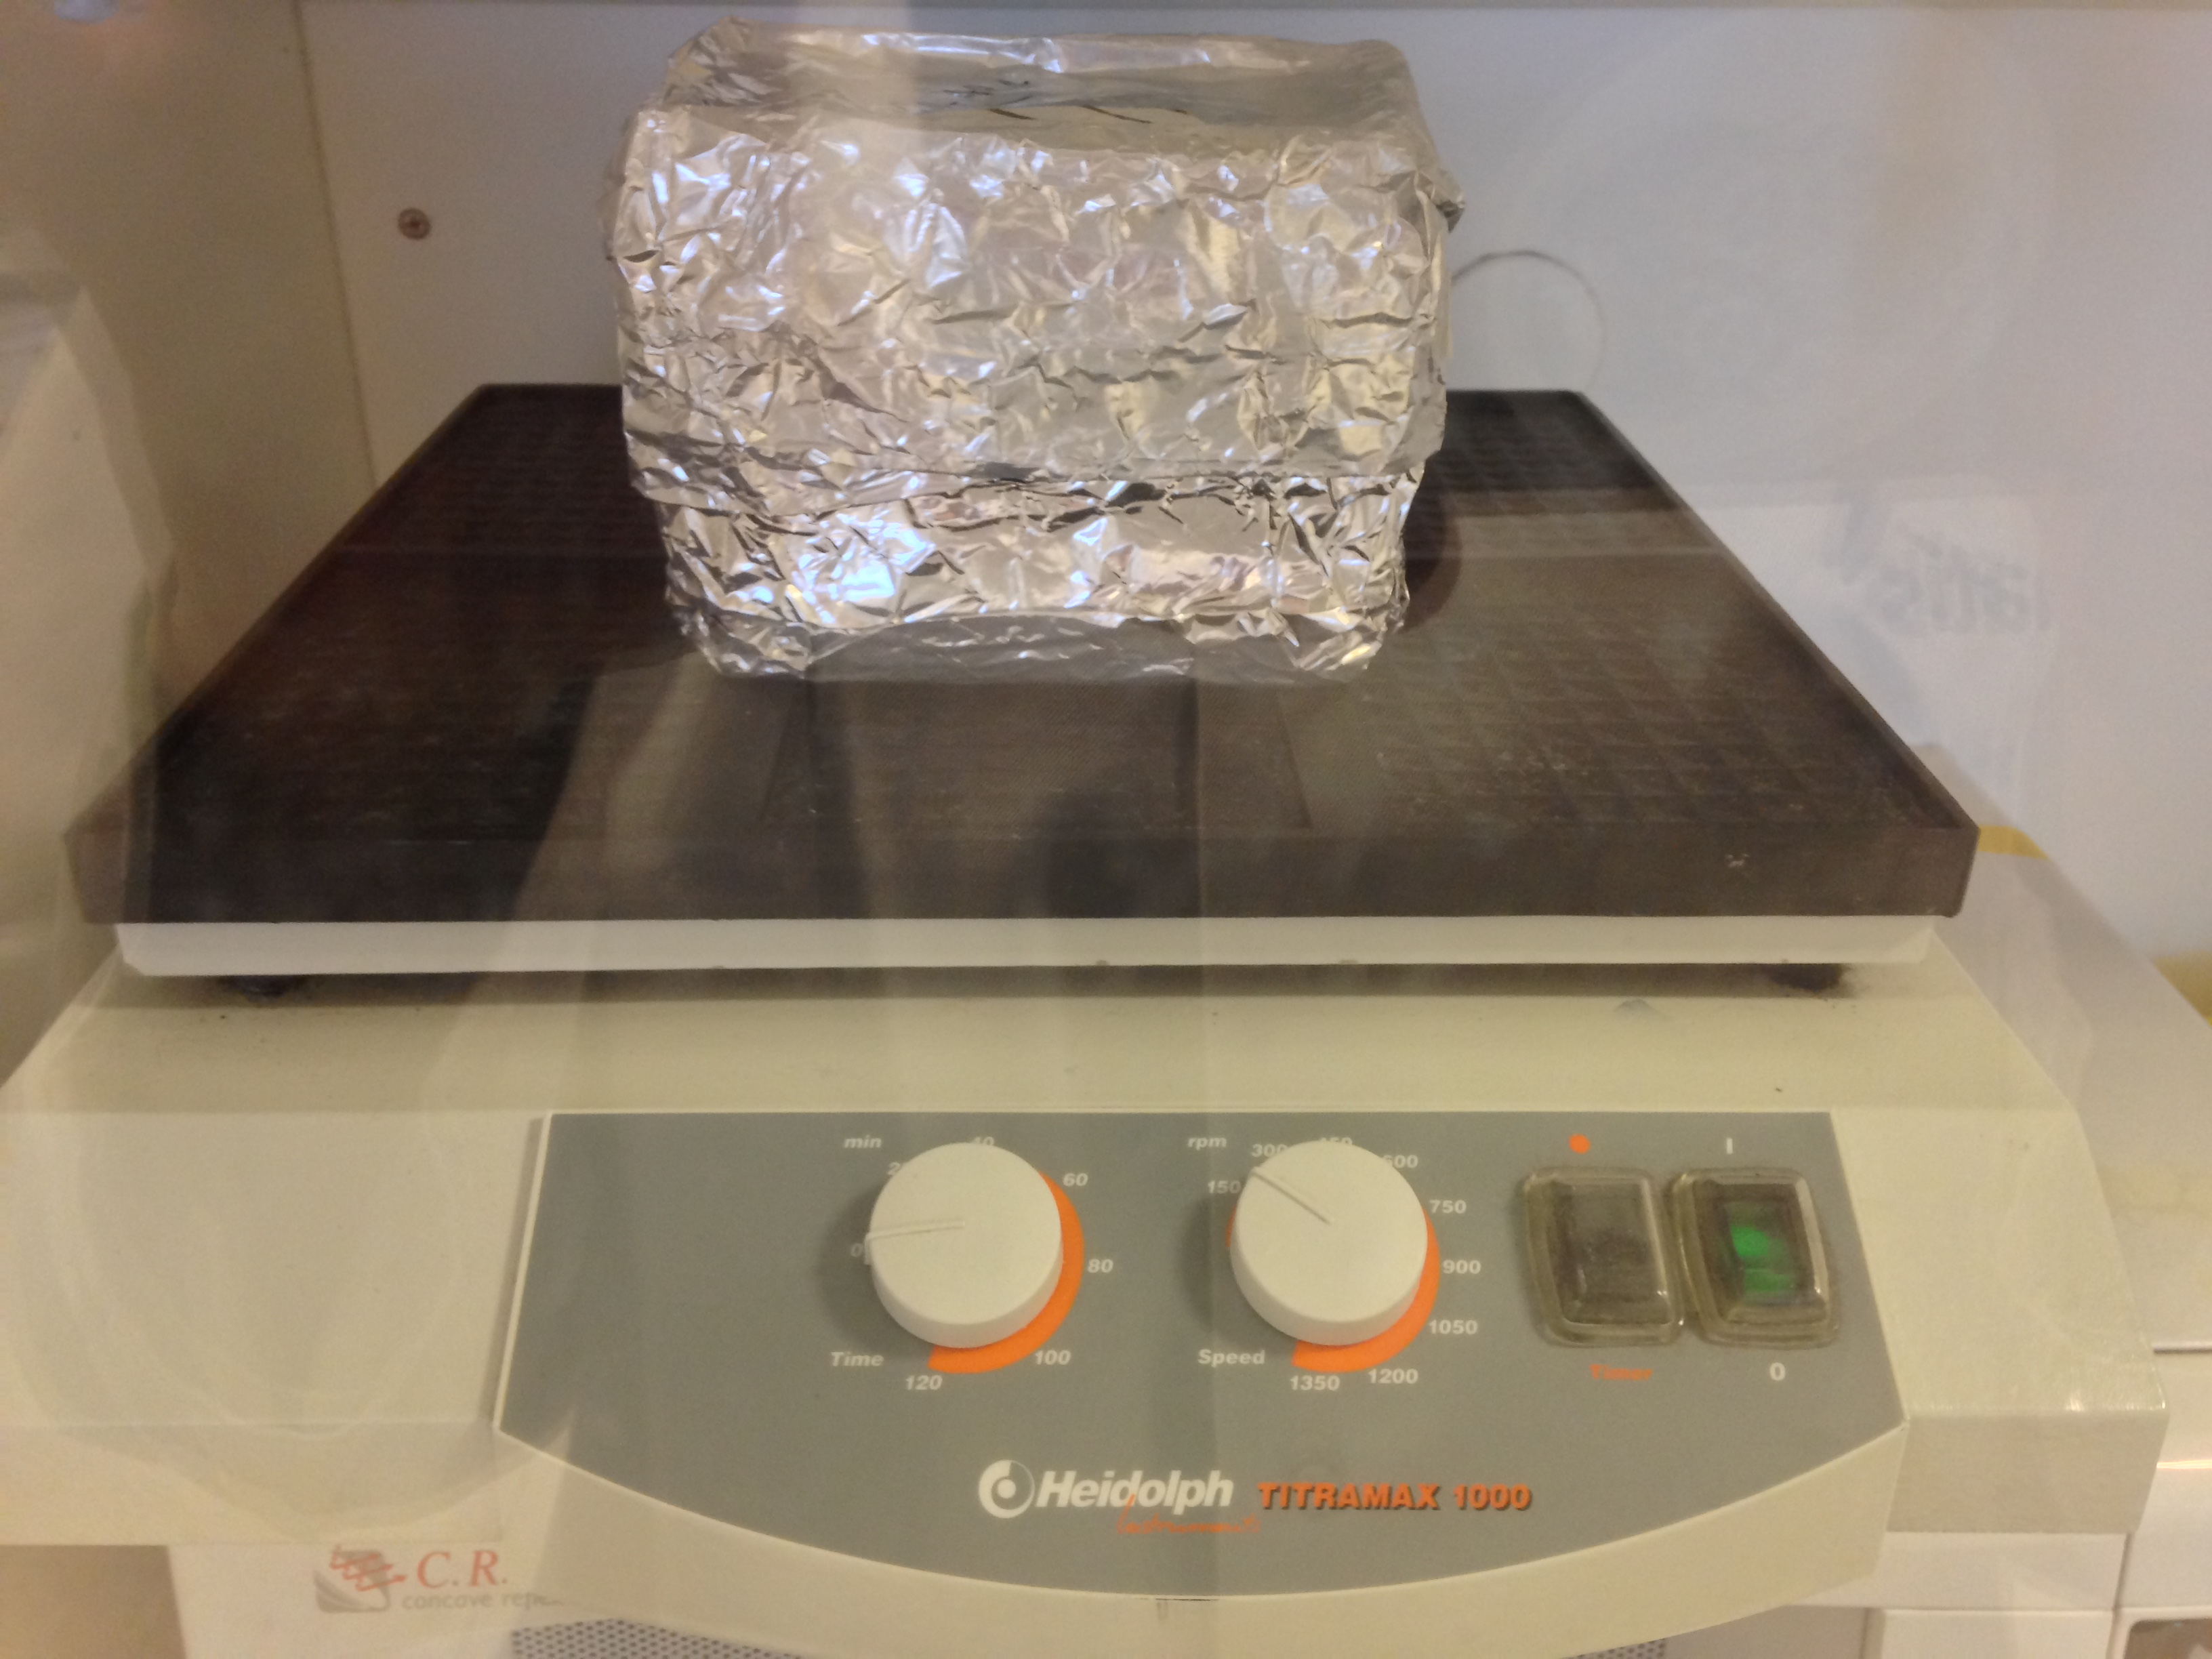
\includegraphics[width=\textwidth]{graphics/pic/20180315_sybr_gold_incubation.JPG}
        \caption{Protect solution from the light with aluminium foil during incubation}
        \label{sfig:20180315_sybr_gold_incubation}
    \end{subfigure}
    ~ 
    \begin{subfigure}[b]{0.208\textwidth}
        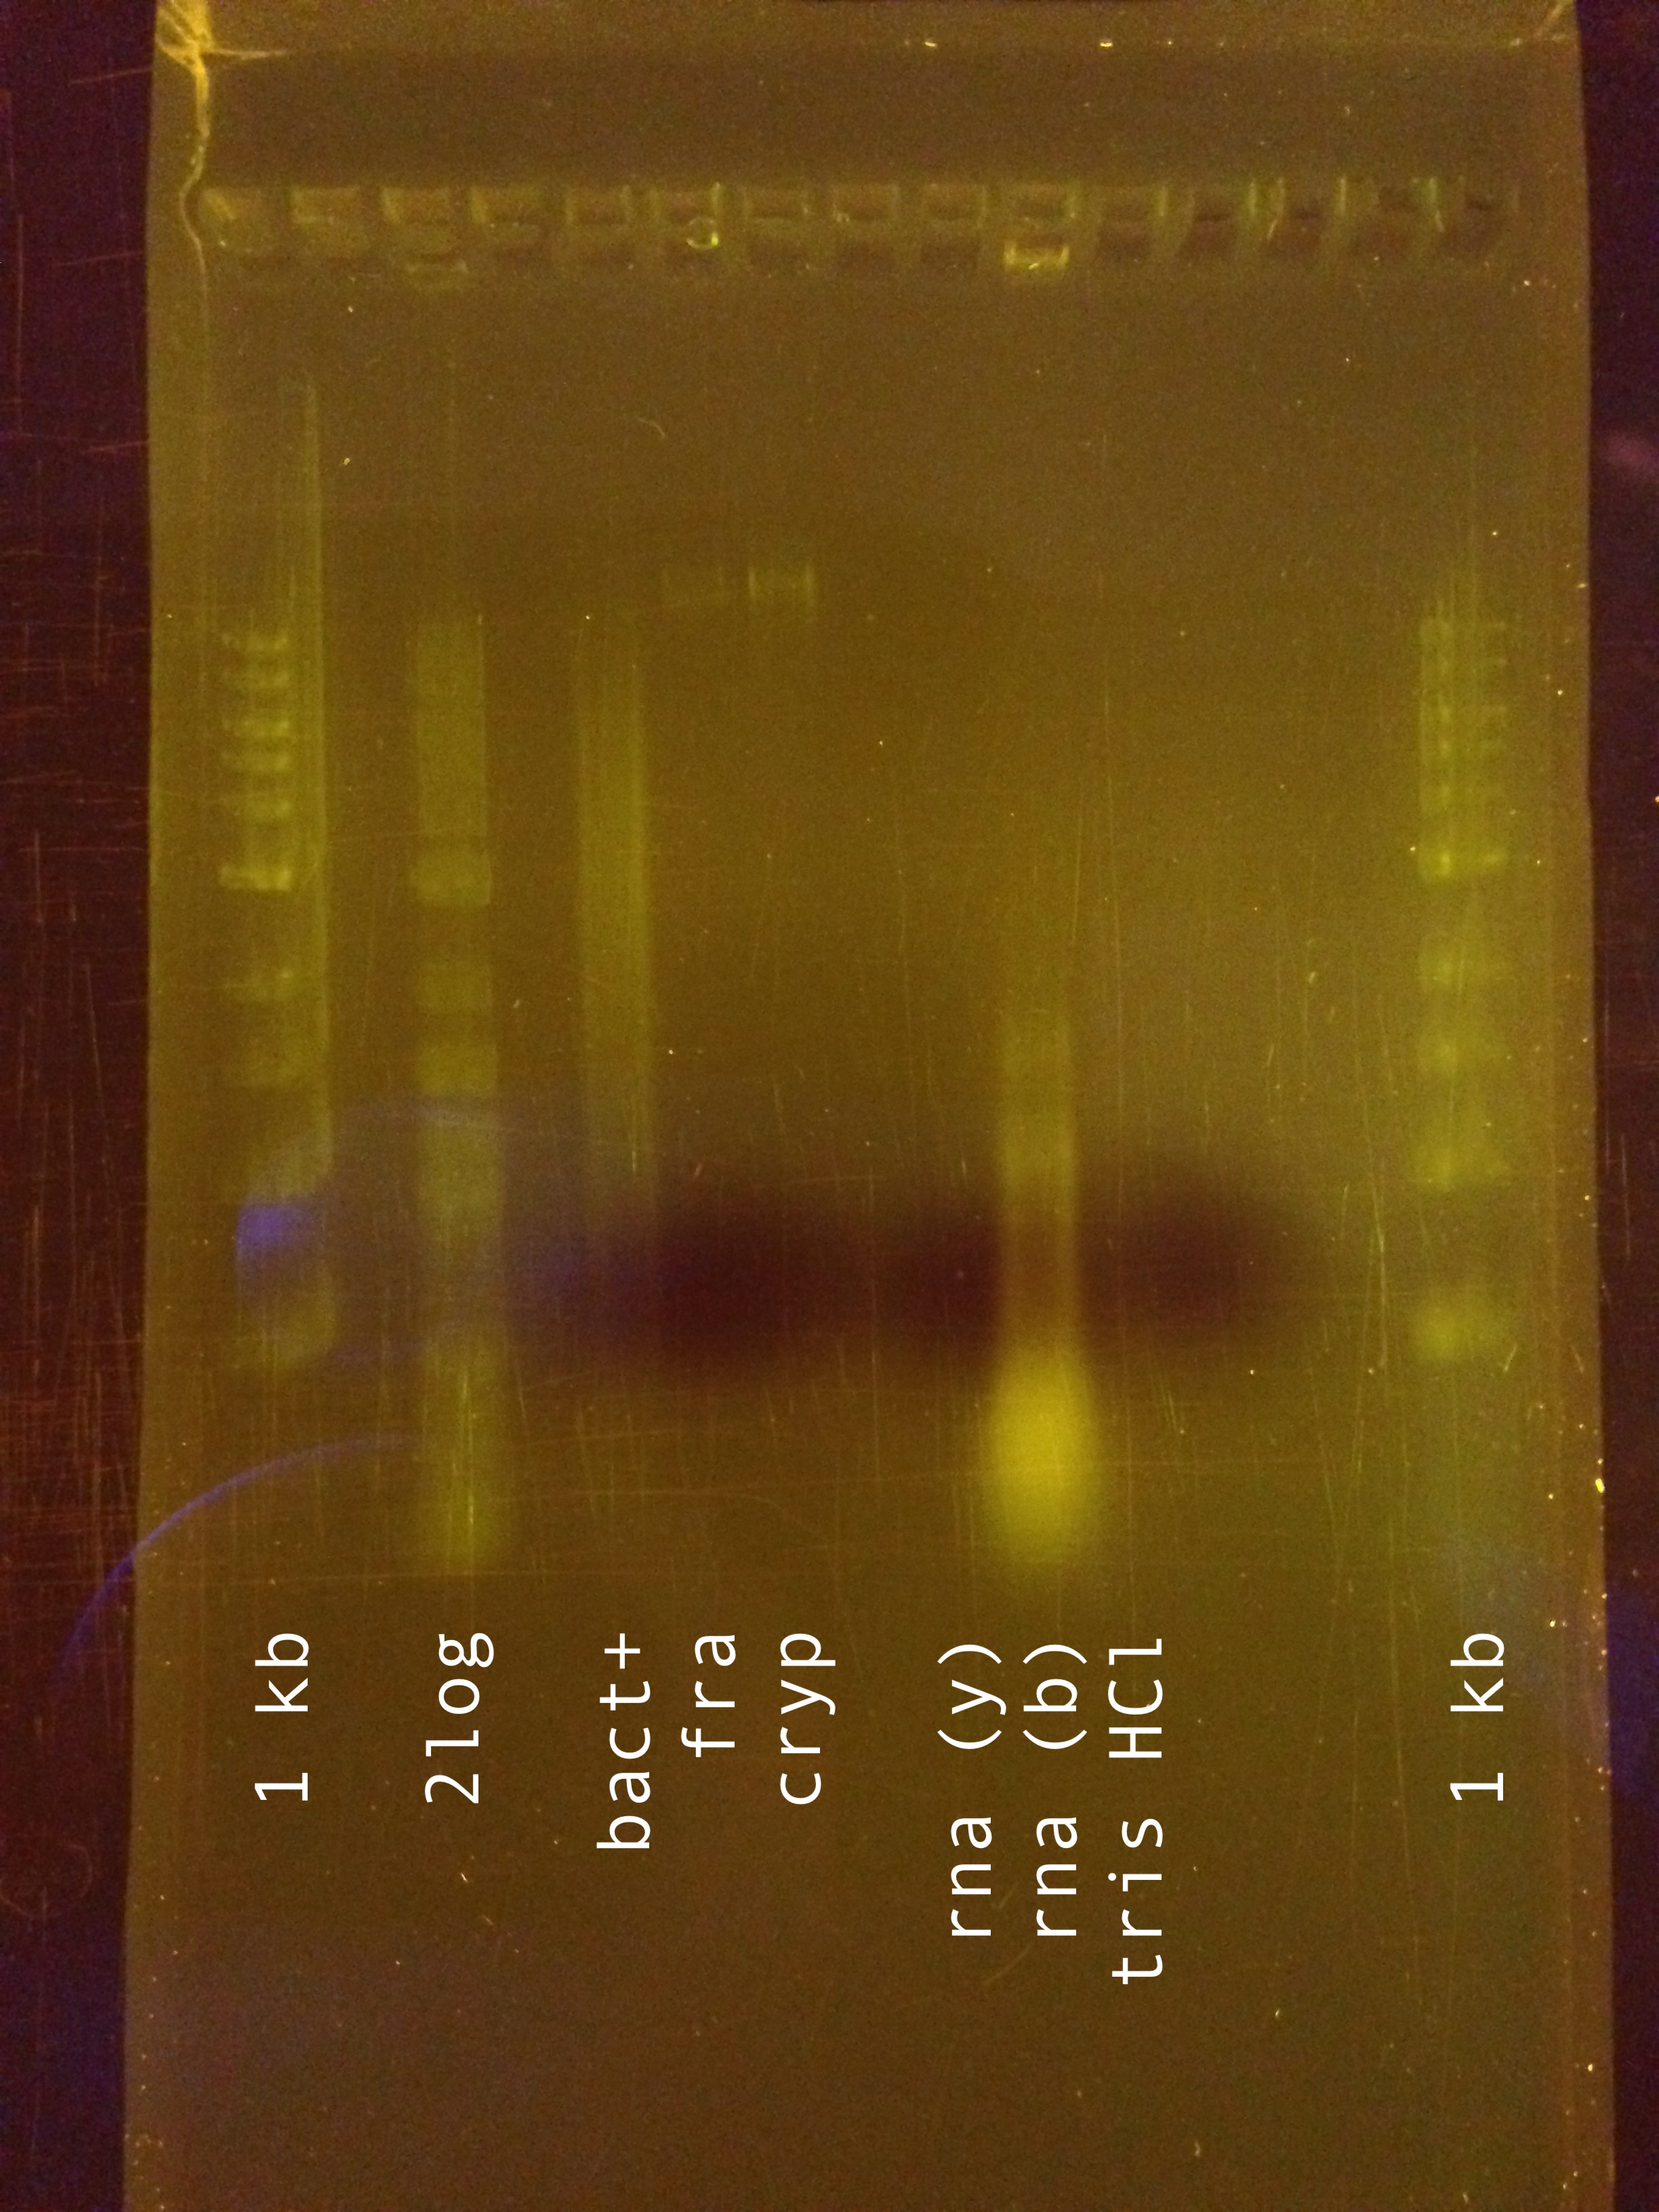
\includegraphics[width=\textwidth]{graphics/pic/20180315_gel_sybr_gold.JPG}
        \caption{Picture of 1\% agarose gel after migration.}
        \label{sfig:20180315_gel_sybr_gold}
    \end{subfigure}
\end{figure}

\subsubsection{Results}

Figure \ref{sfig:20180315_gel_sybr_gold} shows a picture of the gel under \gls{uv} lights after 65 min migration. The ladders are slightly smudged which could be due to the SYBR\cR Gold stain. \sidenote{Pauline Vannier suggests that I just make a test with same migration settings for two ladders with SYBR\cR Safe and Gold to see the difference.} The DNA extracted from AK17 (labelled bact+) is smeared which indicates degradation of the genomic DNA. Since the 1 kb ladder not is sharp and fine, the degradation could have happened during electrophoresis but also during the extraction process or because of repeated freeze-thaw (I use this DNA as positive control for my \gls{pcr} so it has been frozen and thawed a lot of times). \sidenote{If genomic DNA is smeared, using DNase inhibitors while extracting the DNA can prevent degradation of the genomic DNA.} But on the other hand, the genomic DNA extracted from micro-algae cultures (labeled \texttt{fra} and \texttt{cryp}) show sharp band which indicates a rather good integrity of the genomic DNA. Regarding RNA samples, \texttt{RNA (y)} was below the detection level for the Qubit\texttrademark~ so this is no surprise that there is nothing to see. \texttt{RNA (b)} is smeared indicating a poor intergrity of the RNA, but we can still distinguish two bands: the heavier one is approximately at 1.5 kb while the lightest one is at 1 kb. According to Thermo Fisher documentation\sidenote{\url{https://www.thermofisher.com/is/en/home/references/ambion-tech-support/rna-isolation/general-articles/ribosomal-rna-sizes.html}}, for \textit{E. coli} 16S rRNA is 1.5 kb and the 23s rRNA is 2.9 kb. Therefore the two bands observed for the RNA (b) sample could be slightly degraded 16S and 23S rRNA. Finally, the Tris-HCl does not show any band which is a good thing as I just wanted to make sure there was no nucleic acid in the buffer because I had been using it to resuspend my nucleic acids at the end of all my extractions. 

\subsubsection{Conclusion}

SYBR\cR Gold succesfully stains \gls{dna} and \gls{rna} using the procedure performed today so I can now perform this experiment confidently with my RNA and RNA samples extracted from micro-algae culture with AllPrep\cR and MasterPure\texttrademark~ kits.


